\documentclass{article}

\usepackage{pgf}
\usepackage{tikz}
\usetikzlibrary{shapes}
\usepackage{PGFTikzGraph}
\usepackage{subfigure}
\usepackage{multirow}
\usepackage{url}
\usepackage{float}
\usepackage{meta}
\usepackage{amssymb}
\usepackage{amsmath}
\usepackage{epsfig}

\setcounter{page}{1}
\sloppy


\title{Finite Difference Time--Domain Modelling of Metamaterials: GPU Implementation of Cylindrical Cloak} % Please input your paper Title

\name{Attique Dawood} % Please input your name if single author. 

\address{
Department of Electrical Engineering, \\
National University of Computer and Emerging Sciences (FAST), Islamabad, Pakistan \\
E-mail: {\tt attique.dawood@nu.edu.pk}
}

%%%%%%%%%%%%%%%%%%%%%%%%%%%%%%%%%%%%%%%%%%%%%%%%%%%%%%%%%%%%%%%%%%%%%%%%%%
%% If multiple authors (but the same affiliation),                      %%
%% uncomment and edit the lines shown below.                            %%
%% Note that each line must be emphasized {\bf \large } by itself.      %%
%%%%%%%%%%%%%%%%%%%%%%%%%%%%%%%%%%%%%%%%%%%%%%%%%%%%%%%%%%%%%%%%%%%%%%%%%%
%\makeatletter
%\def\name#1{\gdef\@name{#1\\}}
%\makeatother
%\name{{\bf \large  Firstname1 Lastname1, Firstname2 Lastname2, Firstname3 Lastname3,}\\
%      {\bf \large  Firstname4 Lastname4, Firstname5 Lastname5, Firstname6 Lastname6,}\\
%      {\bf \large  and Firstname7 Lastname7}}
%%%%%%%%%%%%%%% End of required multiple authors changes %%%%%%%%%%%%%%%%%

%%%%%%%%%%%%%%%%%%%%%%%%%%%%%%%%%%%%%%%%%%%%%%%%%%%%%%%%%%%%%%%%%%%%%%%%%%
%% If multiple affiliations, uncomment and edit the lines shown below.  %%
%% Note that each line must be emphasized {\bf \large } by itself.      %%
%%%%%%%%%%%%%%%%%%%%%%%%%%%%%%%%%%%%%%%%%%%%%%%%%%%%%%%%%%%%%%%%%%%%%%%%%%
%\makeatletter
%\def\name#1{\gdef\@name{#1\\}}
%\makeatother
%\name{{\bf \large  Firstname1 Lastname1$^1$, Firstname2 Lastname2$^2$, Firstname3 Lastname3$^{1,3}$,}\\
%      {\bf \large  Firstname4 Lastname4$^3$, Firstname5 Lastname5$^{3*}$, and Firstname6 Lastname6}$^{1,2,4}$}
%\address{
%$^1$School of Energy and Power Engineering, Heat Transfer University, Xi'an, China \\
%$^2$Institute of Power Engineering, Computational Science Research Center, Jeju, Korea \\
%$^3$Department of Mechanical Engineering, University of Heat Transfer and Fluid Flow, Kyoto, Japan \\
%$^4$Department of Aeronautics and Astronautics, National Fluid Flow University, Tainan, Taiwan \\
%*corresponding author, E-mail: {\tt author@xx.yyy.zzz}
%}
%%%%%%%%%%%%% End of required multiple affiliations changes %%%%%%%%%%%%%%

%
\begin{document}
\maketitle

%
\begin{abstract}
Finite difference time--domain (FDTD) technique can be used to model metamaterials by treating them as dispersive material. Drude or Lorentz model can be incorporated into the standard FDTD algorithm for modelling negative permittivity and permeability. FDTD algorithm is readily parallelisable and can take advantage of GPU acceleration to achieve speed--ups of 5x--50x depending on hardware setup. Metamaterial scattering problems are implemented using dispersive FDTD technique on GPU resulting in performance gain of 10x--15x compared to conventional CPU implementation.
\end{abstract}

%
\section{Introduction}

Standard FDTD algorithm cannot cater for negative values of permittivity or permeability. This is because of the Courant stability criterion. As soon as the permeability or permittivity becomes less than unity the algorithm will not be stable. A metamaterial object can be modelled as a dispersive substance using either the Lorentz or Drude dispersive models. These models can yield negative values of permittivity (or permeability) for certain frequency ranges~\cite{NumericalFDTD-Sibel}. Using these dispersive models, FDTD update equations are modified and permittivity and permeabilities are replaced with terms dependent on frequency of operation.

Two problems are chosen for GPU implementation. First is the electromagnetic wave scattering by a slab with negative permittivity and permeability; also known as DNG (double negative) medium. Second problem is the simulation of cylindrical cloak. An incident Gaussian pulse on DNG slab will undergo dispersion resulting in different frequency components being separated. Refractive index and transmission coefficient are calculated numerically to ascertain the validity of implementation. The cylindrical cloak was first proposed and tested by Pendry et. al. \cite{PendryShurig-MicrowaveCloak}. The first FDTD implementation was by Zhao et. al \cite{Radial-Zhao} and implemented on Comsol, a commercial electromagnetic simulation software. Simulations are implemented on Matlab, C++ and GPU. Performance comparison reveals a 10--15 times increase in performance with GPU implementations. Performance gain is greater for larger problem sizes and greater simulation times.

\section{Drude Dispersion Model}

In ideal conditions the permittivity (and permeability) of a material remain constant for any frequency and throughout the structure of that material. Speed of electromagnetic waves in such a medium remain constant if frequency changes. Additionally, there is no loss in energy as the waves pass through the medium.

In reality, such a material does not exist. Speed of EM waves varies with frequency of operation. Also, there is a loss associated with the material. A material is dispersive\index{dispersive material} if its permittivity or permeability is dependent on frequency~\cite[Ch. 10]{JBSchneiderUFDTD}.

The relative permittivity in Drude model\index{Drude model $\epsilon_r(\omega)$} is given by
\begin{equation}
\centering
\hat{\epsilon_r}(\omega)=\epsilon_\infty-\dfrac{\omega^2_p}{\omega^2-j\gamma\omega}.
\label{er-Drude}
\end{equation}
Where, $\omega_p$ is plasma frequency and $\gamma$ is collision frequency. Setting $\gamma=0$ and $\epsilon_\infty=1$, relative permittivity comes out to be negative for $\omega/\omega_p > 1$ (figure~\ref{DrudeModel_er}). Thus, Drude model can be effectively used to model metamaterials\index{metamaterial} with permittivity or permeability less than one by incorporating it into FDTD update equations.
\begin{figure}[t!]
\centering
\includegraphics[scale=0.55, trim=4cm 8.5cm 4cm 8.5cm, clip]{FigCh03_DrudeModel_er.pdf}
\caption{$\epsilon_r$ plotted against $\omega/\omega_p$ for $\epsilon_\infty=1$ and $\gamma=0$}
\label{DrudeModel_er}
\end{figure}

\section{FDTD Update Equations}

Faraday's Law\index{Faraday's Law} and Ampere's Law\index{Ampere's Law} in differential form are given by
\begin{equation}
\centering
\nabla \times \textbf{E} = - \dfrac{\partial \textbf{B}}{\partial t},
\label{Faraday's Law}
\end{equation}
\begin{equation}
\centering
\nabla \times \textbf{H} = \dfrac{\partial \textbf{D}}{\partial t}.
\label{Ampere's Law}
\end{equation}
From \cite{Yee1966}, the update equations for a wave propagating in $z$ direction are given by
\begin{equation}
\begin{split}
H^{n+\frac{1}{2}}_y \left[k+\frac{1}{2}\right]&=H^{n-\frac{1}{2}}_y \left[k+\frac{1}{2}\right]\\ &+
\dfrac{\Delta t}{\mu \Delta x} \left( E^{n}_x \left[k\right] - E^{n}_x \left[k+1\right] \right),
\end{split}
\label{Hy-1D-Simple-FDTD-Driver}
\end{equation}
\begin{equation}
\begin{split}
E^{n+1}_x \left[k\right]&=E^{n}_x \left[k\right]\\&+ \dfrac{\Delta t}{\epsilon \Delta x} \left( H^{n+\frac{1}{2}}_y \left[k-\frac{1}{2}\right] - H^{n+\frac{1}{2}}_y \left[k+\frac{1}{2}\right] \right).
\end{split}
\label{Ex-1D-Simple-FDTD-Driver}
\end{equation}
In the conventional FDTD algorithm future magnetic field components are first computed from past electric field components (eq. \ref{Hy-1D-Simple-FDTD-Driver}). Using the updated magnetic field components, future electric field components are then calculated (eq. \ref{Ex-1D-Simple-FDTD-Driver}) and the simulation proceeds in a leap--frog manner \cite{Yee1966}.

\section{FDTD Update Equations Based on Drude Model}

Electric flux density and electric field are related by
\begin{equation}
\centering
\textbf{D} = \epsilon \textbf{E}.
\label{D-epsilon-E}
\end{equation}
Where $\epsilon = \epsilon_r\epsilon_0$ and $\epsilon_r$ for Drude model is given by equation \ref{er-Drude}. Substituting Drude model $\epsilon_r$, equation \ref{D-epsilon-E} can be written as
\begin{equation}
\centering
\omega^2\textbf{D}-\gamma(j\omega)\textbf{D} = \epsilon_\infty\omega^2\textbf{E}-\omega^2_p\textbf{E}-\epsilon_\infty \gamma(j\omega)\textbf{E}.
\label{D-epsilonomega-E-frequency-domain}
\end{equation}
Following the treatment of \cite{Radial-Zhao} and \cite{JBSchneiderUFDTD}, frequency domain quantities can be converted to time--domain using the relationships $j\omega \rightarrow \partial/\partial t$ and $\omega^2 \rightarrow - \partial^2/\partial t^2$. Moreover, fields multiplying with $\omega^2_p$ are averaged in time. Second--order difference scheme is used, both for single and double derivatives to keep all the terms in accordance with the second--order nature of whole expression. This will result in easier implementation. The final form is given by
\begin{equation}
\begin{split}
E^{n+1}_x&=a_e\left(D^{n+1}_x-2D^n_x+D^{n-1}_x\right)\\&+b_e\left(D^{n+1}_x-D^{n-1}_x\right)
+c_e\left(2E^n_x-E^{n-1}_x\right)\\&+d_e\left(2E^n_x+E^{n-1}_x\right)+e_e E^{n-1}_x.
\end{split}
\label{2nd-order-D-E-final-form}
\end{equation}
This is also known as the auxiliary update equation for electric field where $a_e$--$e_e$ are scalars given by
\begin{equation}
\begin{split}
\nonumber & a_e=4/g,~b_e=\gamma\left(2\Delta t\right)/g,~c_e=4\epsilon_0\epsilon_\infty/g,\\
\nonumber & d_e=-\epsilon_0\omega^2_{p}\left(\Delta t\right)^2/g,~e_e=\epsilon_0\epsilon_\infty \gamma_e\left(2\Delta t\right)/g,\\
\nonumber & g=4\epsilon_0\epsilon_\infty+\epsilon_0\omega^2_{p}\left(\Delta t\right)^2+\epsilon_0\epsilon_\infty \gamma \left(2\Delta t\right)
\end{split}
\label{1D-Drude-E-scalars}
\end{equation}
A similar procedure can be carried out to obtain auxiliary update equation for magnetic field.
\begin{equation}
\begin{split}
H^{n+1}_y&=a_m\left(B^{n+1}_y-2B^n_y+B^{n-1}_y\right)\\&+b_m\left(B^{n+1}_y-B^{n-1}_y\right)
+c_m\left(2H^n_y-H^{n-1}_y\right)\\&+d_m\left(2H^n_y+H^{n-1}_y\right)+e_m H^{n-1}_y.
\end{split}
\label{2nd-order-B-H-final-form}
\end{equation}
For a wave propagating in $z$ direction, FDTD update equations\index{FDTD!update equations} are
\begin{equation}
B^{n+1}_y(k)=B^n_y(k)+\dfrac{\Delta t}{\Delta z}\left(E^n_x(k)-E^n_x(k+1)\right)
\label{1D-B-Update-Equation}
\end{equation}
and
\begin{equation}
D^{n+1}_x(k)=D^n_x(k)+\dfrac{\Delta t}{\Delta z}\left(H^{n+1}_y(k-1)-H^{n+1}_y(k)\right).
\label{1D-D-Update-Equation}
\end{equation}
Equations \ref{1D-B-Update-Equation} and \ref{1D-D-Update-Equation} drive the FDTD algorithm which give future values of $By$ and $Dx$ from past fields. Equations \ref{2nd-order-D-E-final-form} and \ref{2nd-order-B-H-final-form} are auxiliary equations which give future fields $H_y$ and $E_x$ at $n+1$. A dry run without any scatterer is carried out before actual simulation to record incident fields. After simulation any post--processing is done to calculate required parameters like refractive index. The whole algorithm is depicted in figure~\ref{1D-DNG-Algorithm}.
\begin{figure}[htbp]
\centering
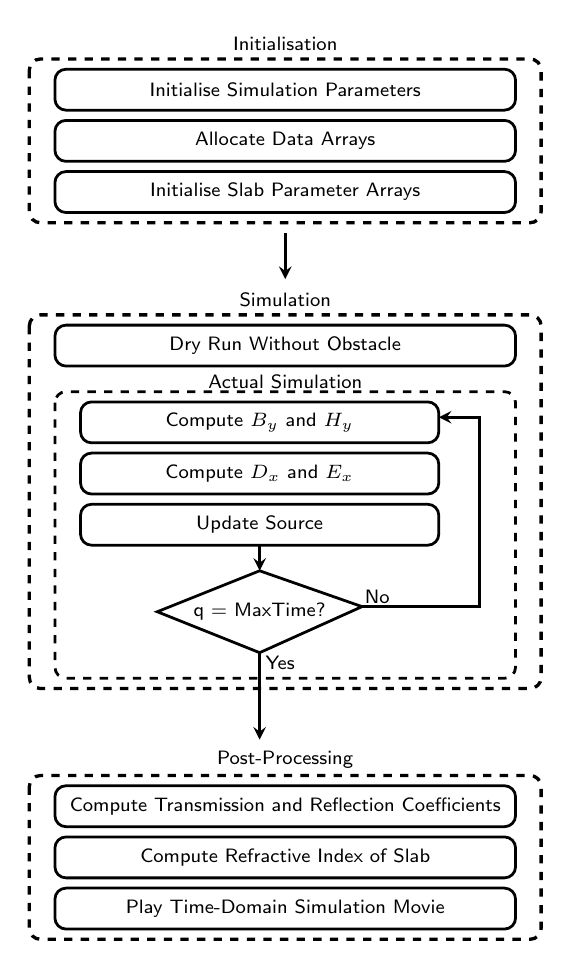
\begin{tikzpicture}[xscale=0.65,yscale=0.65,font=\scriptsize]
	% Initialisation.
	\draw (5cm,0.1cm) node {\textsf{Initialisation}};
	% Large dashed rectangle.
	\draw[line width=1.2pt, rounded corners, dashed] (0cm,-0.2cm) rectangle (10cm,-3.4cm);
	% Simulation parameters.
	\draw[line width=1pt, rounded corners] (0.5cm,-0.4cm) rectangle (9.5cm,-1.2cm);
	\draw (5cm,-0.8cm) node {\textsf{Initialise Simulation Parameters}};
	% Allocate data arrays.
	\draw[line width=1pt, rounded corners] (0.5cm,-1.4cm) rectangle (9.5cm,-2.2cm);
	\draw (5cm,-1.8cm) node {\textsf{Allocate Data Arrays}};
	% Initialise slab parameter arrays.
	\draw[line width=1pt, rounded corners] (0.5cm,-2.4cm) rectangle (9.5cm,-3.2cm);
	\draw (5cm,-2.8cm) node {\textsf{Initialise Slab Parameter Arrays}};
	\draw[line width=1pt, ->, >=stealth] (5cm,-3.6cm) -- (5cm,-4.5cm);

	% Simulation.
	\draw (5cm,-4.9cm) node {\textsf{Simulation}};
	% Large dashed rectangle.
	\draw[line width=1.2pt, rounded corners, dashed] (0cm,-5.2cm) rectangle (10cm,-12.5cm);
	% Dry run without obstacle.
	\draw[line width=1pt, rounded corners] (0.5cm,-5.4cm) rectangle (9.5cm,-6.2cm);
	\draw (5cm,-5.8cm) node {\textsf{Dry Run Without Obstacle}};
	% Actual Simulation.
	\draw[line width=1pt, rounded corners, dashed] (0.5cm,-6.7cm) rectangle (9.5cm,-12.3cm);
	\draw (5cm,-6.5cm) node {\textsf{Actual Simulation}};
	% Compute H fields.
	\draw[line width=1pt, rounded corners] (1.0cm,-6.9cm) rectangle (8.0cm,-7.7cm);
	\draw (4.5cm,-7.3cm) node {\textsf{Compute $B_y$ and $H_y$}};
	% Compute E fields.
	\draw[line width=1pt, rounded corners] (1.0cm,-7.9cm) rectangle (8.0cm,-8.7cm);
	\draw (4.5cm,-8.3cm) node {\textsf{Compute $D_x$ and $E_x$}};
	% Apply source.
	\draw[line width=1pt, rounded corners] (1.0cm,-8.9cm) rectangle (8.0cm,-9.7cm);
	\draw (4.5cm,-9.3cm) node {\textsf{Update Source}};
	\draw[line width=1pt, ->, >=stealth] (4.5cm,-9.7cm) -- (4.5cm,-10.2cm);
	% Diamond.
	\draw[line width=1pt] (4.5cm,-10.2cm) -- (2.5cm,-11cm) -- (4.5cm,-11.8cm) -- (6.5cm,-10.9cm) -- cycle;
	\draw (4.5cm,-11cm) node {\textsf{q = MaxTime?}};
	% No?
	\draw[line width=1pt, ->, >=stealth] (6.5cm,-10.9cm) -- (8.8cm,-10.9cm) -- (8.8cm,-7.2cm) -- (8.0cm,-7.2cm);
	\draw (6.8cm,-10.7cm) node {\textsf{No}};
	% Yes?
	\draw[line width=1pt, ->, >=stealth] (4.5cm,-11.8cm) -- (4.5cm,-12.7cm) -- (4.5cm,-12.7cm) -- (4.5cm,-13.5cm);
	\draw (4.9cm,-12.0cm) node {\textsf{Yes}};

	% Post-processing.
	\draw (5cm,-13.9cm) node {\textsf{Post-Processing}};
	% Large dashed rectangle.
	\draw[line width=1.2pt, rounded corners, dashed] (0cm,-14.2cm) rectangle (10cm,-17.4cm);
	% Transmission/Reflection coefficient calculations.
	\draw[line width=1pt, rounded corners] (0.5cm,-14.4cm) rectangle (9.5cm,-15.2cm);
	\draw (5cm,-14.8cm) node {\textsf{Compute Transmission and Reflection Coefficients}};
	% Refractive index calculations.
	\draw[line width=1pt, rounded corners] (0.5cm,-15.4cm) rectangle (9.5cm,-16.2cm);
	\draw (5cm,-15.8cm) node {\textsf{Compute Refractive Index of Slab}};
	% Simulation movie.
	\draw[line width=1pt, rounded corners] (0.5cm,-16.4cm) rectangle (9.5cm,-17.2cm);
	\draw (5cm,-16.8cm) node {\textsf{Play Time-Domain Simulation Movie}};
\end{tikzpicture}
\caption{FDTD algorithm}
\label{1D-DNG-Algorithm}
\end{figure}
\section{GPU Considerations}
With the evolution of 3D graphics arose a need for faster computing means to handle real--time graphics processing. The graphics processing unit or GPU\index{GPU} was originally meant to act as a separate processor to handle graphics computations. A modern GPU has several hundred small processors that can work in parallel. Generally, these processors are referred to as shaders. The idea is to divide a problem into smaller sub--problems meant to execute in parallel. To take advantage of GPU acceleration a problem must have either task--parallel or data--parallel nature.
\subsection{Task--Parallelism\index{parallelism!task}}
In task--parallelism computation consist of several independent tasks that run concurrently. These tasks may be completely unrelated but the end result is dependent on their outputs. Consider summation of a series, where we want to compute the value of $e^x$ from Taylor series. The mathematical expression is given by
\begin{equation}
e^x = 1+\dfrac{x^1}{1!}+\dfrac{x^2}{2!}+\dfrac{x^3}{3!}+\dfrac{x^4}{4!}+\dfrac{x^5}{5!}+\dfrac{x^6}{6!}+...+\dfrac{x^n}{n!}
\label{eq:ex-Taylor-Series}
\end{equation}

A single--threaded\index{threading!single} conventional implementation would have to calculate all the terms one--by--one and then sum up the result in the end. However, in a multi--threaded\index{threading!multi} implementation, each thread would calculate only one term. All the treads will perform their computation in parallel and the end result is then summed up. The computation--intensive task of calculating factorials and higher powers of $x$ is parallelised and results in significant reduction of computation time.
\subsection{Data--Parallelism\index{parallelism!data}}
In data--parallelism same operation is performed on individual elements of data. A simple example is that of scalar matrix multiplication. Consider an array of size $n$ being multiplied with a scalar constant $c$. The result of each multiplication can be calculated independently by assigning a separate thread for the task. This is illustrated in figure \ref{fig:Data-Parallelism} where input array is \texttt{A[]} and resultant array is \texttt{B[]}. Data--parallelism applies to any scenario where values in resultant data array only depends on values from input array. FDTD\index{FDTD!data--parallelism} is a good example of data--parallelism and a GPU implementation can take advantage of accelerated computing.
\begin{figure}[t!]
\centering
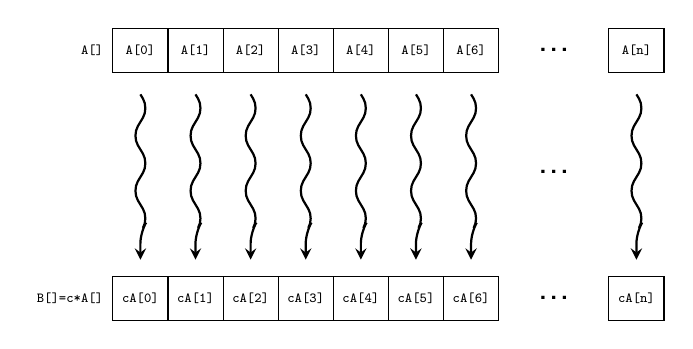
\begin{tikzpicture}[xscale=0.70,yscale=0.70,font=\tiny]
	\newcommand{\Xdisp}{0cm}
	\newcommand{\Ydisp}{0cm}
	% Array A.
	\coordinate [label=left:\texttt{A[]}] (ArrayA) at (\Xdisp,\Ydisp+0.4cm);
	\foreach \x in {0cm,1cm,2cm,3cm,4cm,5cm,6cm,9cm}
		\draw (\x, \Ydisp) rectangle (\x+1cm,\Ydisp+0.8cm);
	\foreach \x/\t in {0.5cm/A[0],1.5cm/A[1],2.5cm/A[2],3.5cm/A[3],4.5cm/A[4],5.5cm/A[5],6.5cm/A[6],9.5cm/A[n]}
		\coordinate [label=center:\texttt{\t}] (Thread\t) at (\x,\Ydisp+0.4cm);
	% Dots.
	\coordinate [label=center:\textsf{{\Large ...}}] (Dots1) at (8cm,\Ydisp+0.4cm);
	% Threads.
	\renewcommand{\Ydisp}{-0.4cm}
	\foreach \x in {0.5cm,1.5cm,2.5cm,3.5cm,4.5cm,5.5cm,6.5cm,9.5cm}
		\draw[thick, rounded corners, ->, >=stealth] (\x+0cm,\Ydisp+0cm) -- (\x+0.15cm,\Ydisp-0.25cm) -- (\x-0.15cm,\Ydisp-0.75cm) -- (\x+0.15cm,\Ydisp-1.25cm) -- (\x-0.15cm,\Ydisp-1.75cm) -- (\x+0.15cm,\Ydisp-2.25cm) -- (\x+0cm,\Ydisp-2.5cm) -- (\x+0cm,\Ydisp-3cm);
	% Dots.
	\coordinate [label=center:\textsf{{\Large ...}}] (Dots2) at (8cm,\Ydisp-1.4cm);
	% Array B.
	\renewcommand{\Ydisp}{-4.5cm}
	\coordinate [label=left:\texttt{B[]=c*A[]}] (ArrayB) at (\Xdisp,\Ydisp+0.4cm);
	\foreach \x in {0cm,1cm,2cm,3cm,4cm,5cm,6cm,9cm}
		\draw (\x, \Ydisp) rectangle (\x+1cm,\Ydisp+0.8cm);
	\foreach \x/\t in {0.5cm/cA[0],1.5cm/cA[1],2.5cm/cA[2],3.5cm/cA[3],4.5cm/cA[4],5.5cm/cA[5],6.5cm/cA[6],9.5cm/cA[n]}
		\coordinate [label=center:\texttt{\t}] (Thread\t) at (\x,\Ydisp+0.4cm);
	% Dots.
	\coordinate [label=center:\textsf{{\Large ...}}] (Dots3) at (8cm,\Ydisp+0.4cm);
\end{tikzpicture}
\caption{Data--parallelism}
\label{fig:Data-Parallelism}
\end{figure}
\section{Simulation of 1D DNG Slab}
\subsection{Problem Specification}
An electromagnetic wave travelling in $z$ direction is incident on a slab with negative values of permittivity and permeability (DNG)\index{DNG} at the frequency of operation \cite{DNG-Ehud-Ziol}. Sinusoidal wave\index{source!sinusoidal}, Gaussian pulse\index{source!Gaussian pulse} and Ricker wavelet\index{source!Ricker wavelet} are used as sources. Transmission\index{coefficient!transmission ($\tau$)} and reflection\index{coefficient!reflection ($\Gamma$)} coefficients are calculated at the air--slab interface. Refractive index of slab\index{refractive index ($n$)} for a range of frequencies is also computed. By varying parameters, the simulation can be scaled to any desired frequency or wavelength.
\subsection{Simulation Results}
The simulation is run for both lossless and lossy cases with sinusoidal\index{source!sinusoidal}, Gaussian\index{source!Gaussian pulse} and Ricker\index{source!Ricker wavelet} wavelet sources. The slab parameters are set such that at frequency of operation, $f_0$, the permittivity and permeability of slab are both negative and result in a refractive index $n=-1$.
\subsection{Simulation Parameters}
The number of spatial steps is set as $4096$ and simulation is run for $4\times 4096$ time steps. The slab is located between steps $1365$ and $2731$. $\Delta z$ or spatial step is set as $3$ mm and time step, $\Delta t$, is set as $50$ ps. Frequency of operation is $f_0=0.1953125$ GHz and Courant number\index{Courant number ($S_c$)} for this configuration comes out to be $S_c=0.5$. In order to obtain relative permittivity and permeability of $-1$ at required $f_0$, plasma frequencies are set as $\omega^2_{pm}=\omega^2_{pe}=2\times(2\pi f_0)^2$ with $\epsilon_\infty=\mu_\infty=1$. First order absorbing boundary condition (ABC) are applied on fields at end points.
\subsection{Incident and Transmitted Fields}
Simulation with Gaussian pulse\index{source!Gaussian pulse} reveals that low frequency components are reflected at the interface which is confirmed from the transmission and reflection coefficients obtained for the air--slab interface. At $f_0$, the transmission coefficient is $1$ and there are no reflections when a sinusoidal source\index{source!sinusoidal} with $f_0$ is incident on the slab. Under steady--state conditions, transmitted wave inside the slab has negative phase velocity while energy is propagating in $+\hat{z}$ direction as expected.
\subsection{Refractive Index}
Following \cite{DNG-Ehud-Ziol}, the refractive index\index{refractive index ($n$)} was calculated from
\begin{equation}
n_{FDTD} = \dfrac{1}{jk_0(z_1-z_2)}log\left|\dfrac{E_x(\omega,z_2)}{E_x(\omega,z_1)}\right|.
\label{Refractive-Index-FDTD}
\end{equation}
Where, $k_0$ was the wave number\index{wave number ($k_0$)} set as $\omega_0/c$ and the fields were recorded at locations $z_1=1415\Delta z$ and $z_2=1424\Delta z$. For both, Gaussian\index{source!Gaussian pulse} pulse and Ricker\index{source!Ricker wavelet} wavelet, $Re(n)$ was $-1$ at $f_0$ while $Im(n)$ was sufficiently close to $0$.
\begin{figure}[t!]
\centering
\includegraphics[scale=0.55, trim=3.5cm 8.7cm 4.5cm 8.85cm, clip]{Figures/FigCh03_IncidentFieldGaussian.pdf}
\caption{Incident Gaussian pulse}
\label{1DDNG-IncidentField-Gaussian}
\end{figure}
\begin{figure}[t!]
\centering
\includegraphics[scale=0.55, trim=3.5cm 8.7cm 4.5cm 8.85cm, clip]{Figures/FigCh03_TransmissionReflectionCoefficient.pdf}
\caption{Transmission and reflection coefficients}
\label{1DDNG-Transmission-Reflection-Coefficient}
\end{figure}
\begin{figure}[t!]
\centering
\includegraphics[scale=0.55, trim=3.5cm 8.7cm 4.5cm 8.85cm, clip]{Figures/FigCh03_TransmittedField.pdf}
\caption{Transmitted Gaussian pulse}
\label{1DDNG-Transmitted-Gaussian-Pulse}
\end{figure}
\begin{figure}[t!]
\centering
\includegraphics[scale=0.55, trim=3.5cm 8.7cm 4.5cm 8.85cm, clip]{Figures/FigCh03_TransmittedFieldBeyondSlab.pdf}
\caption{Transmitted Gaussian pulse beyond slab}
\label{1DDNG-Transmitted-Gaussian-Pulse-Beyond-Slab}
\end{figure}
\begin{figure}[t!]
\centering
\subfigure{\includegraphics[scale=0.55, trim=3.5cm 8.7cm 4.5cm 8.85cm, clip]{Figures/FigCh03_RefractiveIndex.pdf}}
\subfigure{\includegraphics[scale=0.55, trim=3.5cm 8.7cm 4.5cm 8.85cm, clip]{Figures/FigCh03_RefractiveIndexZoomed.pdf}}
\caption{Refractive index}
\label{1DDNG-Refractive-Index}
\end{figure}
\begin{figure}[t!]
\centering
\includegraphics[scale=0.55, trim=3.5cm 8.7cm 4.5cm 8.75cm, clip]{Figures/FigCh03_1DDNGSteadyStateLossless.pdf}
\caption{Steady-state under lossless conditions}
\label{1DDNG-SteadyState-Lossless}
\end{figure}
\begin{figure}[t!]
\centering
\includegraphics[scale=0.55, trim=3.5cm 8.7cm 4.5cm 8.75cm, clip]{Figures/FigCh03_1DDNGSteadyStateLossy.pdf}
\caption{Steady-state under lossy conditions}
\label{1DDNG-SteadyState-Lossy}
\end{figure}
\section{Simulation of 2D DNG Slab}
\subsection{Update Equations}
The most common 2D configurations are $TE^z$\index{polarisation!$TE^z$} or $TM^z$\index{polarisation!$TM^z$} polarisation where the problem space is confined to $xy$--plane. In $TE^z$, electric field components are transverse to $z$--axis and vice versa. For 2D simulation of DNG slab, $TM^z$ polarisation is assumed. The field components of interest would be $E_z$, $H_x$ and $H_y$. Following the approach for 1D case FDTD update equations are
\begin{equation}
\begin{split}
D^{n+1}_z \left[i,j\right]=&D^{n}_z \left[i,j\right]+\dfrac{\Delta t}{\Delta}\left(H^{n+\frac{1}{2}}_y\left[i+\frac{1}{2},j\right]\right.\\
&\left.-H^{n+\frac{1}{2}}_y \left[i-\frac{1}{2},j\right]-H^{n+\frac{1}{2}}_x \left[i,j+\frac{1}{2}\right]\right.\\
&\left.+H^{n+\frac{1}{2}}_x \left[i,j-\frac{1}{2}\right]\right),
\end{split}
\label{eq:Dz-2D-FDTD-TMz}
\end{equation}
\begin{equation}
\begin{split}
B^{n+\frac{1}{2}}_x \left[i,j+\frac{1}{2}\right]=&B^{n-\frac{1}{2}}_x \left[i,j+\frac{1}{2}\right]\\& + \dfrac{\Delta t}{\Delta} \left(-E^{n}_z \left[i,j+1\right] + E^{n}_z \left[i,j\right] \right)
\end{split}
\label{eq:Bx-2D-FDTD-TMz}
\end{equation}
and
\begin{equation}
\begin{split}
B^{n+\frac{1}{2}}_y \left[i+\frac{1}{2},j\right]=&B^{n-\frac{1}{2}}_y \left[i+\frac{1}{2},j\right]\\& + \dfrac{\Delta t}{\Delta} \left( E^{n}_z \left[i+1,j\right] - E^{n}_z \left[i,j\right] \right).
\end{split}
\label{eq:By-2D-FDTD-TMz}
\end{equation}
It is important to note here that DNG slab medium is assumed anisotropic. The auxiliary update equations\index{FDTD!auxiliary update equation} (\ref{2nd-order-B-H-final-form} and \ref{2nd-order-D-E-final-form}) to obtain electric and magnetic fields, $E_v$ and $H_v$ ($v\in x,y,z$), from corresponding flux densities, $D_v$ and $B_v$, remain unchanged.
\subsection{Simulation Geometry}
The DNG slab interface is perpendicular to incident plane wave\index{plane wave} propagating in $+y$ direction. Periodic boundary conditions (PBC)\index{boundary condition!periodic (PBC)} are applied at $x=0$ and $x=x_{max}$. In $y$ direction the grid is terminated at both ends by perfectly matched layer (PML)\index{boundary condition!PML} to absorb any incoming waves. The solution geometry is depicted in figure \ref{fig:2D-DNG-Geometry}. The arrangement of field nodes is shown in figure \ref{fig:2D-DNG-Field-Nodes}.  Magnetic field components are updated first and then used to update electric field.

The solution space is bounded in $y$ direction at both ends by $H_x$ which acts as the boundary for PML. $H_x$ at these end points is set to 0 so that any out--going fields are reflected back into PML. Essentially, the $j$ size of $H_x$ arrays is one greater than $H_y$ and $E_z$ arrays.
\subsection{Simulation Parameters and Results}
The solution space is 512 cells in both $x$ and $y$ directions without taking into account the width of PML, which is 50 cells wide. The plane wave source is located 10 cells from the lower PML layer. The spatial and temporal steps are set as $\Delta x=\Delta y=\Delta=3$ mm and $\Delta t=50$ ps, respectively; with a Courant number of 0.5\index{Courant number ($S_c$)}. Frequency of operation is $f_0=1.5625$ GHz. The DNG slab parameters are same as in the case of 1D DNG simulation.

Figure \ref{fig:2DDNG-Refractive-Index} shows the refractive index\index{refractive index ($n$)} obtained for a range of frequencies with a Gaussian pulse excitation. Again, real part of refractive index at $f_0$ is close to -1, whereas, imaginary part is close to 0.
\begin{figure}[t!]
\centering
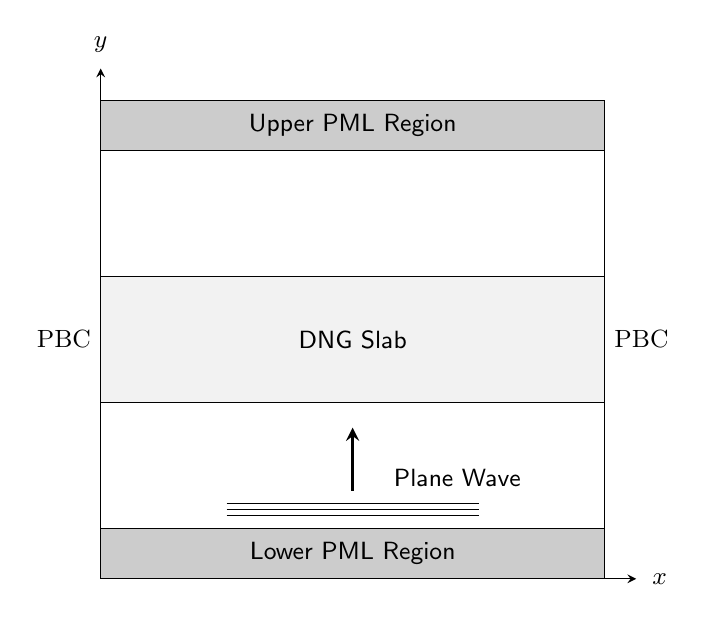
\begin{tikzpicture}[xscale=0.8,yscale=0.8,font=\small]
	\newcommand{\LeftX}{0cm}
	\newcommand{\MidX}{4cm}
	\newcommand{\RightX}{8cm}
	\newcommand{\PMLw}{0.8cm}
	\newcommand{\DomainY}{6.0cm}
	\newcommand{\SlabStartY}{2.0cm+\PMLw}
	\newcommand{\SlabEndY}{4.0cm+\PMLw}
	% x-axis.
	\draw[->, >=stealth] (\LeftX,0cm) -- (\RightX+0.5cm,0cm);
	\coordinate [label=right:$x$] (x-axis) at (\RightX+0.6cm,0cm);
	% y-axis.
	\draw[->, >=stealth] (\LeftX,0cm) -- (\LeftX,2*\PMLw+\DomainY+0.5cm);
	\coordinate [label=above:$y$] (y-axis) at (\LeftX,2*\PMLw+\DomainY+0.6cm);
	% PBCs.
	\coordinate [label=right:PBC] (PBCright) at (\RightX,\PMLw+3.0cm);
	\coordinate [label=left:PBC] (PBCleft) at (\LeftX,\PMLw+3.0cm);
	% Lower PML Region.
	\draw[fill=gray!40!white] (\LeftX,0cm) rectangle (\RightX,\PMLw);
	\coordinate [label=center:\textsf{Lower PML Region}] (LowerPML) at (\MidX,0.4cm);
	% Solution Region.
	\draw (\LeftX,\PMLw) rectangle (\RightX,\PMLw+\DomainY);
	% Upper PML Region.
	\draw[fill=gray!40!white] (\LeftX,\PMLw+\DomainY) rectangle (\RightX,2*\PMLw+\DomainY);
	\coordinate [label=center:\textsf{Upper PML Region}] (UpperPML) at (\MidX,\PMLw+\DomainY+0.4cm);
	% Slab.
	\draw[fill=gray!10!white] (\LeftX,\SlabStartY) rectangle (\RightX,\SlabEndY);
	\coordinate [label=center:\textsf{DNG Slab}] (DNGSlab) at (\MidX,\PMLw+3.0cm);
	% Plane wave.
	\draw (\LeftX+2.0cm,\PMLw+0.2cm) -- (\RightX-2.0cm, \PMLw+0.2cm);
	\draw (\LeftX+2.0cm,\PMLw+0.3cm) -- (\RightX-2.0cm, \PMLw+0.3cm);
	\draw (\LeftX+2.0cm,\PMLw+0.4cm) -- (\RightX-2.0cm, \PMLw+0.4cm);
	\draw[line width=1.1pt, ->, >=stealth] (\MidX,\PMLw+0.6cm) -- (\MidX,\PMLw+1.6cm);
	\coordinate [label=right:\textsf{Plane Wave}] (PlaneWave) at (\MidX+0.5cm,\PMLw+0.8cm);
\end{tikzpicture}
\caption{Simulation geometry}
\label{fig:2D-DNG-Geometry}
\end{figure}
\begin{figure}[t!]
\centering
\vspace{-0.5cm}
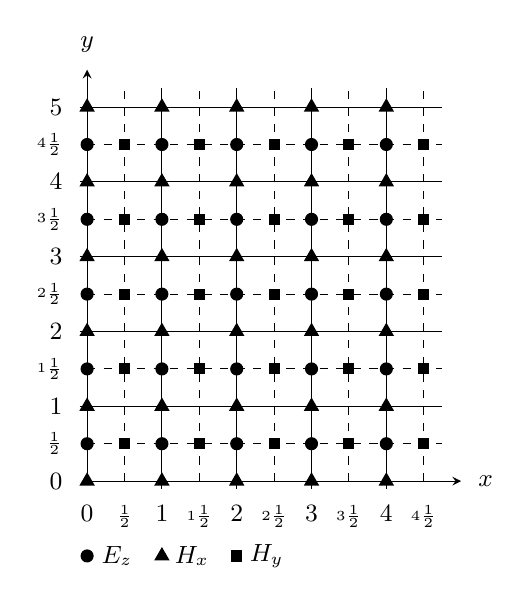
\begin{tikzpicture}[xscale=0.95,yscale=0.95,font=\small]
	\newcommand{\LeftX}{0cm}
	\newcommand{\RightX}{5cm}
	\newcommand{\LowY}{0cm}
	\newcommand{\HighY}{5.5cm}
	% x-axis.
	\draw[->, >=stealth] (\LeftX,\LowY) -- (\RightX,\LowY);
	\coordinate [label=right:$x$] (x-axis) at (\RightX+0.1cm,\LowY);
	% y-axis.
	\draw[->, >=stealth] (\LeftX,\LowY) -- (\LeftX,\HighY);
	\coordinate [label=above:$y$] (y-axis) at (\LeftX,\HighY+0.1cm);
	% Drawing vertical grid lines.
	\foreach \x in {1cm,2cm,3cm,4cm}
		\draw (\x,\LowY-0.1cm) -- (\x,\HighY-0.25cm); % Solid lines at +1 intervals.
	\foreach \x in {0.5cm,1.5cm,2.5cm,3.5cm,4.5cm}
		\draw[dashed] (\x,\LowY) -- (\x,\HighY-0.25cm); % Dashed lines at 1/2 intervals.
	% Drawing horizontal grid lines.
	\foreach \y in {1cm,2cm,3cm,4cm,5cm}
		\draw (\LeftX-0.1cm,\y) -- (\RightX-0.25cm,\y); % Solid lines at +1 intervals.
	\foreach \y in {0.5cm,1.5cm,2.5cm,3.5cm,4.5cm}
		\draw[dashed] (\LeftX,\y) -- (\RightX-0.25cm,\y); % Dashed lines at 1/2 intervals.
	% Drawing nodes.
	\foreach \x in {0cm,1cm,2cm,3cm,4cm}
		\foreach \y in {0.5cm,1.5cm,2.5cm,3.5cm,4.5cm}
			\filldraw (\x,\y) circle (0.08cm); % Ez nodes.
	\foreach \x in {0.5cm,1.5cm,2.5cm,3.5cm,4.5cm}
		\foreach \y in {0.5cm,1.5cm,2.5cm,3.5cm,4.5cm}
			\node[fill=black,regular polygon, regular polygon sides=4,inner sep=0.05cm] at (\x,\y) {}; % Hy nodes.
	\foreach \x in {0cm,1cm,2cm,3cm,4cm}
		\foreach \y in {0cm,1cm,2cm,3cm,4cm,5cm}
			\node[fill=black,regular polygon, regular polygon sides=3,inner sep=0.04cm] at (\x,\y) {}; % Hx nodes.
	% +1 Text for x-axis.
	\foreach \x/\t in {0cm/0,1cm/1,2cm/2,3cm/3,4cm/4}
		\coordinate [label=below:$\t$] (\t) at (\x,\LowY-0.2cm);
	% 1/2 Text for x-axis.
	\foreach \x/\t in {0.5cm/ ,1.5cm/1,2.5cm/2,3.5cm/3,4.5cm/4}
		\coordinate [label=below:{\tiny $\t\frac{1}{2}$}] (\t) at (\x,\LowY-0.2cm);
	% +1 Text for y-axis.
	\foreach \y/\t in {0cm/0,1cm/1,2cm/2,3cm/3,4cm/4,5cm/5}
		\coordinate [label=left:$\t$] (\t) at (\LeftX-0.2cm,\y);
	% 1/2 Text for y-axis.
	\foreach \y/\t in {0.5cm/ ,1.5cm/1,2.5cm/2,3.5cm/3,4.5cm/4}
		\coordinate [label=left:{\tiny $\t\frac{1}{2}$}] (\t) at (\LeftX-0.2cm,\y);
	% Legend
	\filldraw (\LeftX+0cm,\LowY-1cm) circle (0.08cm); % Ez.
	\coordinate [label=center:$E_z$] (EzLegend) at (\LeftX+0.4cm,\LowY-1cm);
	\node[fill=black,regular polygon, regular polygon sides=3,inner sep=0.04cm] at (\LeftX+1cm,\LowY-1cm) {}; % Hx.
	\coordinate [label=center:$H_x$] (HxLegend) at (\LeftX+1.4cm,\LowY-1cm);
	\node[fill=black,regular polygon, regular polygon sides=4,inner sep=0.05cm] at (\LeftX+2cm,\LowY-1cm) {}; % Hy.
	\coordinate [label=center:$H_y$] (HxLegend) at (\LeftX+2.4cm,\LowY-1cm);
\end{tikzpicture}
\caption{Arrangement of field nodes}
\label{fig:2D-DNG-Field-Nodes}
\end{figure}
\begin{figure}[t!]
\centering
\subfigure{\includegraphics[scale=0.55, trim=3.5cm 8.7cm 4.5cm 8.85cm, clip]{Figures/FigCh03_2DDNGRefractiveIndex.pdf}}
\subfigure{\includegraphics[scale=0.55, trim=3.5cm 8.7cm 4.5cm 8.85cm, clip]{Figures/FigCh03_2DDNGRefractiveIndexZoomed.pdf}}
\caption{Refractive index of 2D DNG slab}
\label{fig:2DDNG-Refractive-Index}
\end{figure}
\section{FDTD Modelling of Lossless Cylindrical Cloak}
\subsection{The Electromagnetic Invisibility Cloak\index{cloak}}
It is well known that we can only see things when light bounces off them and reaches our eyes. This is the reason why transparent objects can sometimes be difficult to spot, like window panes. If we can somehow make light bend around the corners of an object so that it continues on its trajectory then that object will appear invisible. Invisibility has, for ages, remained confined to only fiction books but in modern day world of optical transformations and artificially engineered materials, this no longer is a mystery.

An electromagnetic cloak at microwave frequencies was proposed and tested for the first time by Pendry et. al. \cite{PendryShurig-MicrowaveCloak}. The cloak is cylindrical in shape meant to hide a circular object. This is probably the simplest implementation sufficient for proof of concept. To bend light around the circular object the cloaking material must exhibit negative values of permittivity and permeability. The cloaking medium itself is anisotropic. The first attempt at modelling this electromagnetic cloak using the FDTD algorithm was by Zhao et. al. \cite{Radial-Zhao}. Their FDTD implementation was tested using simulation software Comsol\index{Comsol}.
\subsection{Problem Specification}
The implementation in \cite{Radial-Zhao} is for $TE^z$ while in this paper $TM^z$ approach is followed as in the case of DNG slab problems. The cloaking parameters are same and given by
\begin{equation}
\mu_r(r)=\dfrac{r-r_a}{r},
\label{mu-r}
\end{equation}
\begin{equation}
\mu_{\phi}(r)=\dfrac{r}{r-r_a},
\label{mu-phi}
\end{equation}
\begin{equation}
\epsilon_z(r)=\left(\dfrac{r_b}{r_b-r_a}\right)^2\dfrac{r-r_a}{r}.
\label{epsilon-z}
\end{equation}
Here, $r_a$ and $r_b$ are the inner and outer radii of cloaking shell. $r_a$ and $r_b$ are chosen as 0.1 m and 0.2 m respectively. The FDTD implementation is first tested on Matlab, then implemented using C++\index{C++} and finally on GPU. The problem geometry is depicted in figure \ref{fig:2D-Cloak-Geometry}.
\begin{figure}[t!]
\centering
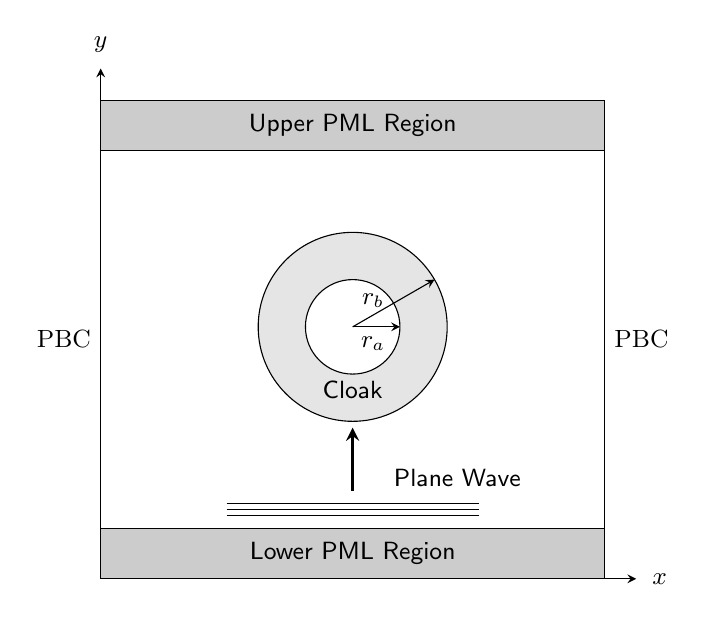
\begin{tikzpicture}[xscale=0.8,yscale=0.8,font=\small]
	\newcommand{\LeftX}{0cm}
	\newcommand{\MidX}{4cm}
	\newcommand{\RightX}{8cm}
	\newcommand{\PMLw}{0.8cm}
	\newcommand{\DomainY}{6.0cm}
	\newcommand{\SlabStartY}{2.0cm+\PMLw}
	\newcommand{\SlabEndY}{4.0cm+\PMLw}
	% x-axis.
	\draw[->, >=stealth] (\LeftX,0cm) -- (\RightX+0.5cm,0cm);
	\coordinate [label=right:$x$] (x-axis) at (\RightX+0.6cm,0cm);
	% y-axis.
	\draw[->, >=stealth] (\LeftX,0cm) -- (\LeftX,2*\PMLw+\DomainY+0.5cm);
	\coordinate [label=above:$y$] (y-axis) at (\LeftX,2*\PMLw+\DomainY+0.6cm);
	% PBCs.
	\coordinate [label=right:PBC] (PBCright) at (\RightX,\PMLw+3.0cm);
	\coordinate [label=left:PBC] (PBCleft) at (\LeftX,\PMLw+3.0cm);
	% Lower PML Region.
	\draw[fill=gray!40!white] (\LeftX,0cm) rectangle (\RightX,\PMLw);
	\coordinate [label=center:\textsf{Lower PML Region}] (LowerPML) at (\MidX,0.4cm);
	% Solution Region.
	\draw (\LeftX,\PMLw) rectangle (\RightX,\PMLw+\DomainY);
	% Upper PML Region.
	\draw[fill=gray!40!white] (\LeftX,\PMLw+\DomainY) rectangle (\RightX,2*\PMLw+\DomainY);
	\coordinate [label=center:\textsf{Upper PML Region}] (UpperPML) at (\MidX,\PMLw+\DomainY+0.4cm);
	% Cloaking shell.
	\draw[fill=gray!20!white] (4cm,4cm) circle (1.5cm);
	\draw[fill=white] (4cm,4cm) circle (0.75cm);
	\coordinate [label=center:\textsf{Cloak}] (Cloak) at (\MidX,3cm);
	\draw[->, >=stealth] (\MidX,4cm) -- (\MidX+0.75cm,4cm);
	\draw[->, >=stealth] (\MidX,4cm) -- (\MidX+1.3005cm,4.75cm);
	\coordinate [label=below:$r_a$] (ra) at (\MidX+0.325cm,4cm);
	\coordinate [label=above:$r_b$] (rb) at (\MidX+0.325cm,4.15cm);
	% Plane wave.
	\draw (\LeftX+2.0cm,\PMLw+0.2cm) -- (\RightX-2.0cm, \PMLw+0.2cm);
	\draw (\LeftX+2.0cm,\PMLw+0.3cm) -- (\RightX-2.0cm, \PMLw+0.3cm);
	\draw (\LeftX+2.0cm,\PMLw+0.4cm) -- (\RightX-2.0cm, \PMLw+0.4cm);
	\draw[line width=1.1pt, ->, >=stealth] (\MidX,\PMLw+0.6cm) -- (\MidX,\PMLw+1.6cm);
	\coordinate [label=right:\textsf{Plane Wave}] (PlaneWave) at (\MidX+0.5cm,\PMLw+0.8cm);
\end{tikzpicture}
\caption{Simulation geometry}
\label{fig:2D-Cloak-Geometry}
\end{figure}
% GPU Implementation
The FDTD update equations for $TM^z$ are completely analogous to those for $TE^z$ presented in \cite{Radial-Zhao}. The update equations for $D_z$, $H_x$ and $H_y$ remain the same as in the case of 2D DNG problem. Figure \ref{fig:Ez-Cloak-SteadyStateLossless} shows $E_z$ under steady--state.
\begin{figure}[t!]
\centering
\includegraphics[scale=0.3]{Figures/FigCh05_Ez_Cloak_SteadyStateLossless.png}
\caption{Ez under steady state for lossless cloak}
\label{fig:Ez-Cloak-SteadyStateLossless}
\end{figure}
All simulation codes are available at~ \url{http://code.google.com/p/computational-electromagnetics/}
\section{Performance Analysis\index{performance analysis}}
\subsection{Hardware and Software Set--up}
Matlab, C++, CUDA and OpenCL implementations are tested with respect to space and time. Operating system, platform/configuration and compiler/toolchain for these implementations are listed in table \ref{Tab:OS-Platform/Configuration-Compiler/Toolchain-for-Testing}. Simulations use \verb|double| data type for arrays on 64 bit optimised platform. The CPU is an Intel Core 2 Duo E8400 @3.00 GHz with 4 GB RAM. For CUDA simulations, GPU is GTX 500 Ti with 192 shaders and 1 GB of memory. Visual C++ 2010 Express is the IDE used on 64 bit Windows 7. The flavour of linux is Fedora 14 64 bit. Hardware and software configuration is listed in table \ref{Tab:Hardware-Software-Configuration-for-Testing}.
\begin{table}[t!]
\begin{center}
\vspace{0.3cm}
	\begin{tabular}{ccc}
	\hline \hline
		\rule{0pt}{2.6ex} & \textbf{Platform/} & \textbf{Compiler/}\\
		& \textbf{Configuration} & \textbf{Toolchain}\\
		\hline
		Matlab \rule{0pt}{2.6ex} & x64 & NA\\
		C++ & x64/O3 & VC++, gcc/g++\\
		OpenCL & x64/O3 & VC++, gcc/g++\\
		CUDA & x64/O3 & nvcc for win/linux\\
	\hline \hline
	\end{tabular}
\end{center}
\caption{Operating system, platform/configuration and compiler/toolchain used for performance testing}
\label{Tab:OS-Platform/Configuration-Compiler/Toolchain-for-Testing}
\end{table}
\begin{table}[t!]
\begin{center}
\vspace{0.3cm}
	\begin{tabular}{ll}
	\hline \hline
		\textbf{CPU} \rule{0pt}{2.6ex}& Intel Core 2 Duo E8400 @3.00 GHz\\
		\textbf{RAM} & 4.00 GB DDR2\\
		\textbf{GPU} & nVidia Geforce GTX 550 Ti 1 GB\\
		\textbf{Matlab} & 2010a 64 bit\\
		\textbf{Linux} & Fedora 14 64 bit\\
		\textbf{Windows} & Win7 64 bit\\
		\textbf{Cygwin} & 64 bit on Win7\\
	\hline \hline
	\end{tabular}
\end{center}
\caption{Hardware and software used for performance testing}
\label{Tab:Hardware-Software-Configuration-for-Testing}
\end{table}
\begin{figure*}[t!]
%\vspace{-0.9cm}
\centering
\mbox{
	\subfigure[Spatial performance times]
	{
	\begin{tikzpicture}[xscale=0.6,yscale=0.6,font=\small]
		\DrawAxes{size}{time~(sec)}
		\GridOn
		\TicksOn
		\XAxisText{0.313cm/32^2}{1.25cm/128^2}{2.5cm/256^2}{3.75cm/384^2}{ 5cm/512^2}{6.25cm/640^2}{7.5cm/768^2}{8.75cm/896^2}{10cm/1024^2}
		\YAxisText{0.00cm/0}{1.00cm/60}{2.00cm/120}{3.00cm/180}{4.00cm/240}{5.00cm/300}{6.00cm/360}{7.00cm/420}{8.00cm/480}
		\YAxisText{9.00cm/540}{10.00cm/600}{}{}{}{}{}{}{}
		% 2D spatial all plots with 256 time steps
		\draw[line width=1.2pt,color=red!40!yellow] (0.31cm,0.019cm) -- (0.63cm,0.025cm) -- (1.3cm,0.048cm) -- (2.5cm,0.2cm) -- (3.8cm,0.59cm) -- ( 5cm,1.2cm) -- (6.3cm,2.1cm) -- (7.5cm,3.3cm) -- (8.8cm,4.4cm) -- (10cm, 6cm);
		\draw[line width=1.2pt,color=red!10!yellow] (0.31cm,0.00082cm) -- (0.63cm,0.0038cm) -- (1.3cm,0.02cm) -- (2.5cm,0.3cm) -- (3.8cm,0.41cm) -- ( 5cm,2.5cm) -- (6.3cm,2.5cm) -- (7.5cm,5.2cm) -- (8.8cm,5.9cm) -- (10cm,9.8cm);
		\draw[line width=1.2pt,color=blue] (0.31cm,0.00087cm) -- (0.63cm,0.0033cm) -- (1.3cm,0.017cm) -- (2.5cm,0.32cm) -- (3.8cm,0.5cm) -- ( 5cm,2.1cm) -- (6.3cm,2.7cm) -- (7.5cm,4.4cm) -- (8.8cm,5.6cm) -- (10cm,8.5cm);
		\draw[line width=1.2pt,color=blue!30!white] (0.31cm,0.0032cm) -- (0.63cm,0.0062cm) -- (1.3cm,0.022cm) -- (2.5cm,0.13cm) -- (3.8cm,0.37cm) -- ( 5cm,2.3cm) -- (6.3cm,2.3cm) -- (7.5cm,4.8cm) -- (8.8cm,5.4cm) -- (10cm,9.2cm);
		\draw[line width=1.2pt,color=gray!70!white] (0.31cm,0.0093cm) -- (0.63cm,0.011cm) -- (1.3cm,0.017cm) -- (2.5cm,0.049cm) -- (3.8cm,0.091cm) -- ( 5cm,0.17cm) -- (6.3cm,0.24cm) -- (7.5cm,0.36cm) -- (8.8cm,0.5cm) -- (10cm,0.66cm);
		\draw[line width=1.2pt,color=pink] (0.31cm,0.013cm) -- (0.63cm,0.013cm) -- (1.3cm,0.017cm) -- (2.5cm,0.046cm) -- (3.8cm,0.095cm) -- ( 5cm,0.18cm) -- (6.3cm,0.25cm) -- (7.5cm,0.36cm) -- (8.8cm,0.45cm) -- (10cm,0.66cm);
		\draw[line width=1.2pt,color=red!70!black] (0.31cm,0.0022cm) -- (0.63cm,0.0027cm) -- (1.3cm,0.0035cm) -- (2.5cm,0.0078cm) -- (3.8cm,0.014cm) -- ( 5cm,0.023cm) -- (6.3cm,0.034cm) -- (7.5cm,0.049cm) -- (8.8cm,0.066cm) -- (10cm,0.085cm);
		\draw[line width=1.2pt,color=red] (0.31cm,0.0067cm) -- (0.63cm,0.0067cm) -- (1.3cm,0.0078cm) -- (2.5cm,0.012cm) -- (3.8cm,0.02cm) -- ( 5cm,0.03cm) -- (6.3cm,0.043cm) -- (7.5cm,0.058cm) -- (8.8cm,0.075cm) -- (10cm,0.097cm);
		\draw[line width=1.2pt,color=green!50!black] (0.31cm,0.0012cm) -- (0.63cm,0.0014cm) -- (1.3cm,0.0021cm) -- (2.5cm,0.0068cm) -- (3.8cm,0.013cm) -- ( 5cm,0.024cm) -- (6.3cm,0.035cm) -- (7.5cm,0.051cm) -- (8.8cm,0.068cm) -- (10cm,0.089cm);
		\draw[line width=1.2pt,color=green] (0.31cm,0.005cm) -- (0.63cm,0.005cm) -- (1.3cm,0.0067cm) -- (2.5cm,0.011cm) -- (3.8cm,0.019cm) -- ( 5cm,0.03cm) -- (6.3cm,0.043cm) -- (7.5cm,0.06cm) -- (8.8cm,0.081cm) -- (10cm,0.1cm);
	\end{tikzpicture}
	}
	\subfigure[Temporal performance times]
	{
	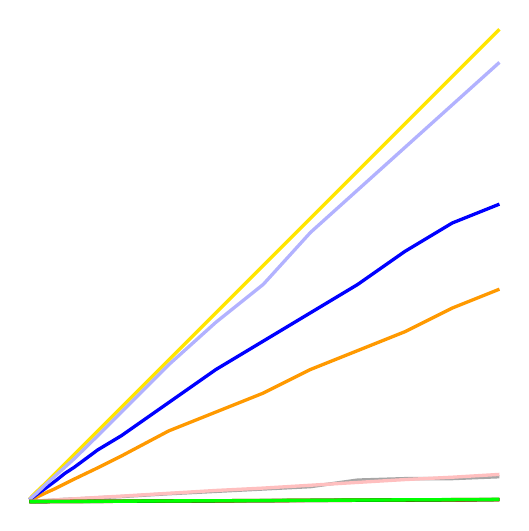
\begin{tikzpicture}[xscale=0.6,yscale=0.6,font=\small]
		\DrawAxes{steps}{time~(sec)}
		\GridOn
		\TicksOn
		\XAxisText{0.05cm/25}{1cm/}{2cm/1000}{3cm/}{4cm/2000}{5cm/}{6cm/3000}{7cm/}{8cm/4000}
		\XAxisText{9cm/}{10cm/5000}{}{}{}{}{}{}{}
		\YAxisText{0.00cm/0}{1.00cm/280}{2.00cm/560}{3.00cm/840}{4.00cm/1120}{5.00cm/1400}{6.00cm/1680}{7.00cm/1960}{8.00cm/2240}
		\YAxisText{9.00cm/2520}{10.00cm/2800}{}{}{}{}{}{}{}
		% ------- 2D temporal with 512^2 size -------
		\draw[line width=1.2pt,color=red!40!yellow] (0.05cm,0.027cm) -- (0.1cm,0.047cm) -- (0.2cm,0.094cm) -- (0.4cm,0.19cm) -- (0.6cm,0.28cm) -- (0.8cm,0.38cm) -- ( 1cm,0.48cm) -- (1.5cm,0.72cm) -- ( 2cm,0.97cm) -- ( 3cm,1.5cm) -- ( 4cm,1.9cm) -- ( 5cm,2.3cm) -- ( 6cm,2.8cm) -- ( 7cm,3.2cm) -- ( 8cm,3.6cm) -- ( 9cm,4.1cm) -- (10cm,4.5cm);
		\draw[line width=1.2pt,color=red!10!yellow] (0.05cm,0.052cm) -- (0.1cm,0.11cm) -- (0.2cm,0.21cm) -- (0.4cm,0.4cm) -- (0.6cm,0.6cm) -- (0.8cm,0.8cm) -- ( 1cm, 1cm) -- (1.5cm,1.5cm) -- ( 2cm, 2cm) -- ( 3cm, 3cm) -- ( 4cm, 4cm) -- ( 5cm, 5cm) -- ( 6cm, 6cm) -- ( 7cm, 7cm) -- ( 8cm, 8cm) -- ( 9cm, 9cm) -- (10cm,10cm);
		\draw[line width=1.2pt,color=blue] (0.05cm,0.046cm) -- (0.1cm,0.076cm) -- (0.2cm,0.15cm) -- (0.4cm,0.29cm) -- (0.6cm,0.44cm) -- (0.8cm,0.6cm) -- ( 1cm,0.73cm) -- (1.5cm,1.1cm) -- ( 2cm,1.4cm) -- ( 3cm,2.1cm) -- ( 4cm,2.8cm) -- ( 5cm,3.4cm) -- ( 6cm, 4cm) -- ( 7cm,4.6cm) -- ( 8cm,5.3cm) -- ( 9cm,5.9cm) -- (10cm,6.3cm);
		\draw[line width=1.2pt,color=blue!30!white] (0.05cm,0.048cm) -- (0.1cm,0.094cm) -- (0.2cm,0.18cm) -- (0.4cm,0.37cm) -- (0.6cm,0.55cm) -- (0.8cm,0.73cm) -- ( 1cm,0.91cm) -- (1.5cm,1.4cm) -- ( 2cm,1.9cm) -- ( 3cm,2.9cm) -- ( 4cm,3.8cm) -- ( 5cm,4.6cm) -- ( 6cm,5.7cm) -- ( 7cm,6.6cm) -- ( 8cm,7.5cm) -- ( 9cm,8.4cm) -- (10cm,9.3cm);
		\draw[line width=1.2pt,color=gray!70!white] (0.05cm,0.014cm) -- (0.1cm,0.01cm) -- (0.2cm,0.016cm) -- (0.4cm,0.026cm) -- (0.6cm,0.038cm) -- (0.8cm,0.053cm) -- ( 1cm,0.059cm) -- (1.5cm,0.086cm) -- ( 2cm,0.11cm) -- ( 3cm,0.17cm) -- ( 4cm,0.22cm) -- ( 5cm,0.27cm) -- ( 6cm,0.32cm) -- ( 7cm,0.46cm) -- ( 8cm,0.49cm) -- ( 9cm,0.49cm) -- (10cm,0.53cm);
		\draw[line width=1.2pt,color=pink] (0.05cm,0.0099cm) -- (0.1cm,0.011cm) -- (0.2cm,0.017cm) -- (0.4cm,0.028cm) -- (0.6cm,0.04cm) -- (0.8cm,0.051cm) -- ( 1cm,0.063cm) -- (1.5cm,0.092cm) -- ( 2cm,0.12cm) -- ( 3cm,0.18cm) -- ( 4cm,0.24cm) -- ( 5cm,0.29cm) -- ( 6cm,0.35cm) -- ( 7cm,0.41cm) -- ( 8cm,0.47cm) -- ( 9cm,0.52cm) -- (10cm,0.58cm);
		\draw[line width=1.2pt,color=red!70!black] (0.05cm,0.003cm) -- (0.1cm,0.0025cm) -- (0.2cm,0.0029cm) -- (0.4cm,0.0037cm) -- (0.6cm,0.0045cm) -- (0.8cm,0.0053cm) -- ( 1cm,0.0062cm) -- (1.5cm,0.0082cm) -- ( 2cm,0.01cm) -- ( 3cm,0.015cm) -- ( 4cm,0.018cm) -- ( 5cm,0.023cm) -- ( 6cm,0.027cm) -- ( 7cm,0.031cm) -- ( 8cm,0.035cm) -- ( 9cm,0.039cm) -- (10cm,0.043cm);
		\draw[line width=1.2pt,color=red] (0.05cm,0.0068cm) -- (0.1cm,0.0041cm) -- (0.2cm,0.0045cm) -- (0.4cm,0.0054cm) -- (0.6cm,0.0063cm) -- (0.8cm,0.0072cm) -- ( 1cm,0.0083cm) -- (1.5cm,0.011cm) -- ( 2cm,0.013cm) -- ( 3cm,0.017cm) -- ( 4cm,0.022cm) -- ( 5cm,0.027cm) -- ( 6cm,0.031cm) -- ( 7cm,0.036cm) -- ( 8cm,0.04cm) -- ( 9cm,0.045cm) -- (10cm,0.05cm);
		\draw[line width=1.2pt,color=green!50!black] (0.05cm,0.0029cm) -- (0.1cm,0.0026cm) -- (0.2cm,0.0031cm) -- (0.4cm,0.0039cm) -- (0.6cm,0.0048cm) -- (0.8cm,0.0057cm) -- ( 1cm,0.0066cm) -- (1.5cm,0.0088cm) -- ( 2cm,0.011cm) -- ( 3cm,0.016cm) -- ( 4cm,0.02cm) -- ( 5cm,0.024cm) -- ( 6cm,0.029cm) -- ( 7cm,0.033cm) -- ( 8cm,0.038cm) -- ( 9cm,0.042cm) -- (10cm,0.047cm);
		\draw[line width=1.2pt,color=green] (0.05cm,0.0045cm) -- (0.1cm,0.0036cm) -- (0.2cm,0.0041cm) -- (0.4cm,0.0051cm) -- (0.6cm,0.006cm) -- (0.8cm,0.0072cm) -- ( 1cm,0.0079cm) -- (1.5cm,0.01cm) -- ( 2cm,0.013cm) -- ( 3cm,0.018cm) -- ( 4cm,0.022cm) -- ( 5cm,0.027cm) -- ( 6cm,0.032cm) -- ( 7cm,0.036cm) -- ( 8cm,0.041cm) -- ( 9cm,0.046cm) -- (10cm,0.051cm);
	\end{tikzpicture}
	}
}
\begin{tikzpicture}
\DrawLegend
\end{tikzpicture}
\caption{Performance comparison}
\label{fig:Peformance-comparison}
\end{figure*}
\section{Conclusions}

The goal of this paper was to analyse GPU performance gain of dispersive FDTD and GPU implementation of lossless cylindrical cloak. It was shown that materials with negative permeability and permittivity can be effectively modelled using Drude dispersive model. The numerical results showed good agreement with theoretical values in the case of DNG slab problem

The 1D and 2D cases of slab problem was then implemented using C++ and GPU. A comprehensive performance analysis showed that GPU was able to perform much better both, as the problem domain and maximum time stepping are increased. For smaller problems, however, it is better to use Matlab or C++ due to data copying overhead associated with GPU implementation.

The lossless case of cylindrical cloak, as presented by Zhao et. al. in \cite{Radial-Zhao}, was implemented using Matlab, C++ and finally on GPU with minor modifications. The simulations showed adequate similarity to accepted results.

\begin{acknowledgement}
I would like to thank Dr. Rashad Ramzan for his guidance.
\end{acknowledgement}
\newpage
\nocite{*}
\bibliographystyle{IEEEtran}
\bibliography{FDTDMETARef}
%\begin{thebibliography}{10}
%%%---
%\bibitem[1]{Zhang10} 
%A.-B. Zhang, C.-D. Kim, E. Yamada, F.G. Smith, 
%The numerical investigation on the turbulent heat transfer, 
%{\em Int. J. Heat Mass Transfer} 12: 345--365, 2010.
%%%---
%\bibitem[2]{Patankar80} 
%S.V. Patankar, 
%{\em Numerical Heat Transfer and Fluid Flow}, 
%Hemisphere Publishers, New York, 1980.
%%%---
%\bibitem[3]{Kays90} 
%W.M. Kays, M.E. Crawford, 
%{\em Heat transfer}, 
%Wiley, New York, pp.256-258, 1990.
%%%---
%\bibitem[4]{Kawa09} 
%Y. Kawaguchi, T. Tsukahara, M. Motozawa, 
%Experimental and numerical investigations of turbulent drag reduction phenomena by additives,
%{\em Proc. aes09},
%Jeju, Korea, pp. 23--32, 2009.
%%%---
%\end{thebibliography}
\end{document}
